\documentclass[pageno]{jpaper}

\newcommand{\IWreport}{2017}
\newcommand{\quotes}[1]{``#1''}


\widowpenalty=9999

\usepackage[normalem]{ulem}
\usepackage{amsmath}

\begin{document}

\title{Solving the Generalized Form of the Game of Set Efficiently}

\author{Steven Takeshita\\Adviser: Zachary Kincaid}

\date{}
\maketitle

\thispagestyle{empty}
\doublespacing
\begin{abstract}
This paper examines three implementations of a solver for the generalized version of the Game of Set. Brute force, SMT solver based, and dynamic algorithm approaches are used to create an efficient solver for the game. Through timing tests, it is shown that though a reduction to the SMT solver should create an efficient solution to the NP complete game, the dynamic algorithm approach yields the fastest solver in many test cases over both the SMT solver and brute force implementations. 
\end{abstract}

\section{Motivation and Goal}

The Game of Set was created in 1974 and published in 1991. The game consists of $3^4 = 81$ unique cards. Each card has 4 properties and one of three values. A valid set of three cards is one in which for each property, they all either have the same or different value. At the beginning of the game, 12 cards are shown, and players must locate valid sets. Once a set is found or no set exists, three new cards are added. The most number of sets collected at the ends win. Therefore, a natural extension of this problem is to determine how fast can we find sets. The goal of my project is to create a solver that locates a set efficiently in practice for a game with $p$ properties and $v$ values. The Game of Set is an interesting problem for dynamic algorithms in that when three new cards are added, the algorithm should be able to build off of previous knowledge. A way to utilize this past information could be helpful in applying similar principles to other problems that could lend itself to dynamic programming. 


\section{Problem Background and Related Work}


The Game of Set has been researched thoroughly for education and as a motivating example for cap sets, but little research exists about solving a generalized version. Chaudhuri et al (2003) proved that the generalized version of Set is in fact NP-Complete through a reduction from perfect-Dimensional Matching, a known NP-Hard problem ~\cite{chaudhuri}.  

This paper proves computational complexity bounds, but does not solve the problem in practice. Solvers do exist on the internet and can be readily found ~\cite{nolte}. Some solvers even employ image processing to identify sets ~\cite{jorquera}. However, the solvers are constrained to have four properties and three values. Therefore, the solver I will build will be able to solve the generic case of Set in which it has $p$ properties and $v$ values.  

\subsection{Problem Definition}

A deck will contain $v^p$ possible cards where the cards have $p$ properties and $v$ values. Initially, $v*p$ cards will be outputted as the starting layout. Identify an arbitrary set of $v$ cards, in which for all properties the values are either the same or all different. Remove this set of size $v$ and count it as another set found, or if no set exists, add $v$ more cards from the remaining $v^p - v$ cards. Find a total of $n$ sets, where $n \leq v^{p-1}$ and each time a set is found $v$ more cards will be immediately added. Therefore, there are 2 update functions that the algorithms must handle. One to add $v$ new cards to the board and the other to remove $v$ cards that formed a set. 

By removing the first set of cards seen, this will simulate real gameplay, in which the goal is to find sets as fast as possible. By finding a generalized $n$ number of sets, as cards are added and removed, the dynamic algorithm will hopefully see some speed up. This further simulates gameplay in which the goal is to find a collection of sets and it is likely that there might not exists sets or sets will be found causing new cards to be added. 

\section{Approach}

Generalizing the Game of Set has been done academically, but no practical solution to locate sets exists. A reduction to SMT creates a solver to theoretically always verify whether a set exists, but this does not verify a set within reasonable time if we consider the the poly-time transformation and the fact that it needs to recalculate a set every time new cards are added, not using information from previous rounds to verify it faster. Therefore, my approach will use previous knowledge of the absence of sets to quickly discover sets in a new showing of cards. Set's changing probabilities of discovering a Set also lends itself to the dynamic algorithm approach. Norvig (2017) showed that on a fresh layout of the game with 12 cards, the ratio of games in which there exists a Set to those that do not contain a set, is 29:1. But as the game plays on, the ratio drops to 15:1, a 50\% less chance of finding a set. For 15 cards, the ratio drops to 4\% of its original ratio ~\cite{norvig}. Therefore, as the game is iteratively played in which Sets are taken out, the game becomes immensely harder. With a dynamic algorithm approach, the solver I build should be able to beat the SMT solver especially with this added difficulty as Sets are removed from the board. 


\section{Reduction to SMT}

\subsection{Set Up}

There exists $v*p$ cards forming a starting board $B$, but in general there will be $n$ cards on a board at any moment. These cards can be represented as vectors where all entries $b_{i,j} \in \{0,1, ... , v-1\}$:

\begin{align}
    B &= \begin{bmatrix}
           b_{1,1} \\
           b_{1,2} \\
           \vdots \\
           b_{1,p}
         \end{bmatrix}
         \begin{bmatrix}
           b_{2,1} \\
           b_{2,2} \\
           \vdots \\
           b_{2,p}
         \end{bmatrix} ... 
          \begin{bmatrix}
           b_{n,1} \\
           b_{n,2} \\
           \vdots \\
           b_{n,p}
         \end{bmatrix}
  \end{align}
  
The SMT Solver will then attempt to find a set of $v$ cards. The satisfying set can be denoted as vectors where $k_{i,j} \in \{0,1, ... , v-1\}$:

\begin{align}
    K &= \begin{bmatrix}
           k_{1,1} \\
           k_{1,2} \\
           \vdots \\
           k_{1,p}
         \end{bmatrix}
         \begin{bmatrix}
           k_{2,1} \\
           k_{2,2} \\
           \vdots \\
           k_{2,p}
         \end{bmatrix} ... 
          \begin{bmatrix}
           k_{v,1} \\
           k_{v,2} \\
           \vdots \\
           k_{v,p}
         \end{bmatrix}
  \end{align}

\subsection{All Different or All Same Constraint}
To correctly identify satisfying, distinct sets that exist from the given cards, we need to create three sets of constraints. The first set of constraints will only be satisfied when the cards found $K$ represent a set, where for all properties, they have either the same or all different value. This constraint can be written as two cases for each property of the cards:

\textbf{The values are all the same for a given property i:} 
\begin{align}
	(k_{1,i} = k_{2,i}) \wedge (k_{2,i} = k_{3,i}) \wedge ... \wedge (k_{v-1,i} = k_{v,i})
\end{align}
\begin{align}
	\bigwedge \limits_{m=1}^{v-1} k_{m,i} = k_{m+1,i}
\end{align}

\textbf{The values are all different for a given property i:}
\begin{multline}
	((k_{1,i} \neq k_{2,i}) \wedge (k_{1,i} \neq k_{3,i}) \wedge ... \wedge (k_{1,i} \neq k_{v,i})) \\
	 \wedge ((k_{2,i} \neq k_{3,i}) \wedge (k_{2,i} \neq k_{4,i}) \wedge ... \wedge (k_{2,i} \neq k_{v,i})) \wedge 
	 ... \wedge (k_{v-1,i} \neq k_{v,i})
\end{multline}

\begin{align}
	\bigwedge \limits_{m=1}^{v-1}  \bigwedge \limits_{j = m+1}^{v} k_{m,i} \neq k_{j,i}
\end{align}


Therefore, we can write more concisely that for all properties of the cards, the values must all be the same or all different:

\begin{align}
	\bigwedge \limits_{i=1}^{p}  \left(  \left( \bigwedge \limits_{m=1}^{v-1}  \bigwedge \limits_{j = m+1}^{v} k_{m,i} \neq k_{j,i} \right)  \bigvee  	 \left(  \bigwedge \limits_{m=1}^{v-1} k_{m,i} = k_{m+1,i} \right) \right)
\end{align}


\subsection{The Cards Must Be From The Board}

The second set of constraints is that the cards selected in the set $K$ must all be from the board $B$, which is of size $n$. This constraint can be encoded into the SMT solver as:

A given card $i$ from $K$ must be from the board $B$:
\begin{multline}
	((k_{i,1} = b_{1,1}) \wedge (k_{i,2} = b_{1,2}) \wedge ... \wedge (k_{i,p} = b_{1,p})) \vee \\
	 ((k_{i,1} = b_{2,1}) \wedge (k_{i,2} = b_{2,2}) \wedge ... \wedge (k_{i,p} = b_{2,p}))  \vee ... \vee \\ ((k_{i,1} = b_{n,1}) \wedge (k_{i,2} = b_{n,2}) \wedge ... \wedge (k_{i,p} = b_{n,p})) 
\end{multline}

Therefore, all cards $i \in K$ must be from the board $B$:
 
\begin{align}
	\bigwedge \limits_{i=1}^{v}  \left( \bigvee \limits_{j = 1}^{n}  \left( \bigwedge \limits_{m=1}^{p}  k_{i,m} = b_{j,m}\right) \right)
\end{align}

\subsection{All Distinct Cards}

We constrain the possible cards in the set to be from $B$, but this includes duplicates. A possible set could be three of the exact same cards and would satisfy the above constraints but does not represent a real set in the game. Therefore, the last constraint is that the cards selected to be in $K$, must all be distinct cards. The cards of a set are considered all distinct if for any two cards, they have at least one property that has a differing value. The constraint can be written as:


%%%% possibly rewrite this better such that for a given card i make sure that the cards above it (ie. j = i+1) are all totally distinct
%%% and then more concisely can write that for all it would be better... pick one

A given card, $i$, differs with respect to at least one property compared to all cards coming after $i:$

\begin{multline}
	((k_{i,1} \neq k_{i+1,1}) \vee (k_{i,2} \neq k_{i+1,2}) \vee ... \vee (k_{i,p} \neq k_{i+1,p}))  \wedge \\
	((k_{i,1} \neq k_{i+2,1}) \vee (k_{i,2} \neq k_{i+2,2}) \vee ... \vee (k_{i,p} \neq k_{i+2,p}))  \wedge ... \wedge \\ 
	((k_{i,1} \neq k_{v,1}) \vee (k_{i,2} \neq k_{v,2}) \vee ... \vee (k_{i,p} \neq k_{v,p})) 
\end{multline}

Written more succinctly:


%\begin{multline}
%	((k_{1,1} \neq k_{2,1}) \vee (k_{1,2} \neq k_{2,2}) \vee ... \vee (k_{1,p} \neq k_{2,p}))  \wedge \\
%	((k_{1,1} \neq k_{3,1}) \vee (k_{1,2} \neq k_{3,2}) \vee ... \vee (k_{1,p} \neq k_{3,p}))  \wedge ... \wedge \\ 
%	((k_{1,1} \neq k_{v,1}) \vee (k_{1,2} \neq k_{v,2}) \vee ... \vee (k_{1,p} \neq k_{v,p})) \wedge \\
%	((k_{2,1} \neq k_{3,1}) \vee (k_{2,2} \neq k_{3,2}) \vee ... \vee (k_{2,p} \neq k_{3,p})) \wedge  ... \wedge \\ 
%	((k_{2,1} \neq k_{v,1}) \vee (k_{2,2} \neq k_{v,2}) \vee ... \vee (k_{2,p} \neq k_{v,p})) \wedge ... \wedge \\
%	((k_{v-1,1} \neq k_{v,1}) \vee (k_{v-1,2} \neq k_{v,2}) \vee ... \vee (k_{v-1,p} \neq k_{v,p})) 
%\end{multline}



\begin{align}
	\bigwedge \limits_{i=1}^{v-1}   \left( \bigwedge \limits_{j=i+1}^{v}   \left( \bigvee \limits_{m = 1}^{p} k_{i,m} \neq k_{j,m} \right)  \right)
\end{align}

\subsection {Condensing Sets}

To ensure that the cards are constrained as much as possible for the domain of the SMT solver, we can say that for every possible set, the cards need to be in sorted order by their first property, and if the values are all the same, then by the sorted by the second property, and so forth if the cards in the set have equivalent value for a given property. This can be encoded as follows: 

\begin{multline}
	(k_{1,1} \leq k_{2,1} \leq ... \leq k_{v,1}) \wedge (   (k_{1,2} \leq k_{2,2} \leq ... \leq k_{v,2})  \vee \neg (k_{1,1} = k_{2,1} = ... = k_{v,1})) \\
	\wedge (   (k_{1,3} \leq k_{2,3} \leq ... \leq k_{v,3})  \vee \neg (k_{1,2} = k_{2,2} = ... = k_{v,2}) \vee \neg (k_{1,1} = k_{2,1} = ... = k_{v,1})) \\
	\wedge ... \wedge (   (k_{1,p} \leq k_{2,p} \leq ... \leq k_{v,p})  \vee \neg (k_{1,p-1} = k_{2,p-1} = ... = k_{v,p-1}) \vee ... \vee \neg (k_{1,1} = k_{2,1} = ... = k_{v,1}))
\end{multline}

Written more compactly:

\begin{align}
	\bigwedge \limits_{i=1}^{p}   \left(  (k_{1,i} \leq k_{2,i} \leq ... \leq k_{v,i}) \bigvee \limits_{j=1}^{i-1}  \left( \neg (k_{1,j} = k_{2,j} = ... = k_{v,j})  \right)   \right)
\end{align}

By building these four constraints (7, 9, 11, 12) from a given board, we can reduce finding an arbitrary set to SMT and use a solver to locate a set efficiently. 

\subsection{Update Functions} 
The solver to find sets must also support two update functions. The first update function of removing cards can be easily encoded into the SMT constraints. Let set $V$ be an arbitrary set that was located by the SMT solver. To remove the set from the board, we can add new constraints such that the new set to be found cannot be equal to any of the cards found in $V$, where $V$ contains $v$ cards. Again, to be a distinct card, at least one property must be differing. This can be written as:

\begin{align}
	\forall k \in K, \forall v \in V \left (k_1 \neq v_1 \vee k_2 \neq v_2 \vee ... \vee k_p \neq v_p \right)
\end{align}

A given card $i$ from $K$ must not be equivalent to a card in $V$:

\begin{multline}
	((k_{i,1} \neq v_{1,1}) \vee (k_{i,2} \neq v_{1,2}) \vee ... \vee (k_{i,p} \neq v_{1,p})) \wedge \\
	 ((k_{i,1} \neq v_{2,1}) \vee (k_{i,2} \neq v_{2,2}) \vee ... \vee (k_{i,p} \neq v_{2,p}))  \wedge ... \wedge \\ ((k_{i,1} \neq v_{v,1}) \vee (k_{i,2} \neq v_{v,2}) \vee ... \vee (k_{i,p} \neq v_{v,p})) 
\end{multline}

All cards $i \in K$ must not be equivalent to a card in $V$:

\begin{align}
	\bigwedge \limits_{i=1}^{v}   \left( \bigwedge \limits_{j=1}^{v}  \left( \bigvee \limits_{m = 1}^{p} k_{i,m} \neq v_{j,m} \right)   \right)
\end{align}




For the second update function in which new cards may be added to the deck, we will need to create a new set of constraints (7, 9, 11) from above. Therefore, this is represents a full reduction to SMT from the Game of Set. 


\section{Implementation}

The simulations for the randomizer and solvers were all written in python. Considering python's lightweight feel and ease of iterating over all variables in a list, makes it the natural extension for representing a deck and board of cards. Therefore, python made the code easier to write up and allowed for helpful language defined shortcuts. 


\subsection{Randomizer}

The randomization algorithm for creating a randomized deck is very important in terms of creating a real life scenario gameplay. Therefore, the algorithm must uniformly distribute all of the cards ($v*p$) initially so that no solver can have an unfair advantage knowing what cards are more likely to come out. To do so, I used a couple of important libraries to ensure randomness and to plot the distribution in order to guarantee its uniform distribution. I used the Random library in python to be able to generate random indices to pull for the beginning board ($v*p$) and for the next $v$ cards when sets are found. I assumed the Random library to be perfectly random. To ensure that the next $v$ cards are always random from the set, I employed the use of a modified version of Fisher Yates Shuffle, creating a Las Vegas algorithm. Fisher Yates Shuffle works by iteratively randomly picking indices from a finite sequence and produces an unbiased permutation \cite{fisher}. To convert the algorithm for use on a deck, I use rejection sampling to determine new cards to add to the board. I create a randomized card and if it is not in the board already and not in the removed cards set, I add it. If it is, I generate another card until I have created $v*p$ cards that are all distinct. Since the algorithm uses a randomized strategy but will always a board, whose cards are all distinct and from the deck with equal probabilities, this is known as a Las Vegas algorithm. To support the update function of removing cards, I append those cards to a set of removed cards. Therefore, when $v$ new cards are to be added, I generate $v$ new random cards through the above algorithm to be added to the board. This yields a randomized $v*p$ starting boards and unbiased drawing of $v$ cards from the deck.

To confirm that this in fact created random beginning boards and new cards, I graphed the distribution of the beginning board for $1000$ trials with $v = 10$ and $p = 10$. I then used numpy to and matplotlib to count all the occurrences of each card and then graph them as a histogram. In Figure~\ref{fig:init1}  and~\ref{fig:init2}, we can see that in both cases (3 properties, 4 values and 4 properties, 5 vales), the distribution of cards that were initially selected to be on the board form a uniform distribution over 10,000 trials.

\begin{figure}[htbb]
\begin{minipage}[b]{0.5\linewidth}
\centering
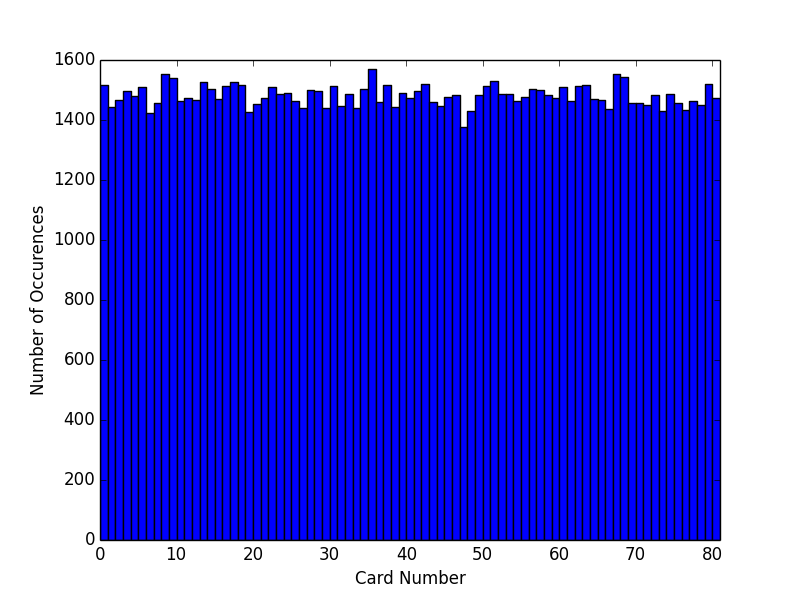
\includegraphics[width=.75\linewidth]{3p4v10000Init.png}
\caption{3 properties, 4 values, 10,000 trials Initial Board Distribution}
\label{fig:init1}
\end{minipage}
\hspace{0.5cm}
\begin{minipage}[b]{0.5\linewidth}
\centering
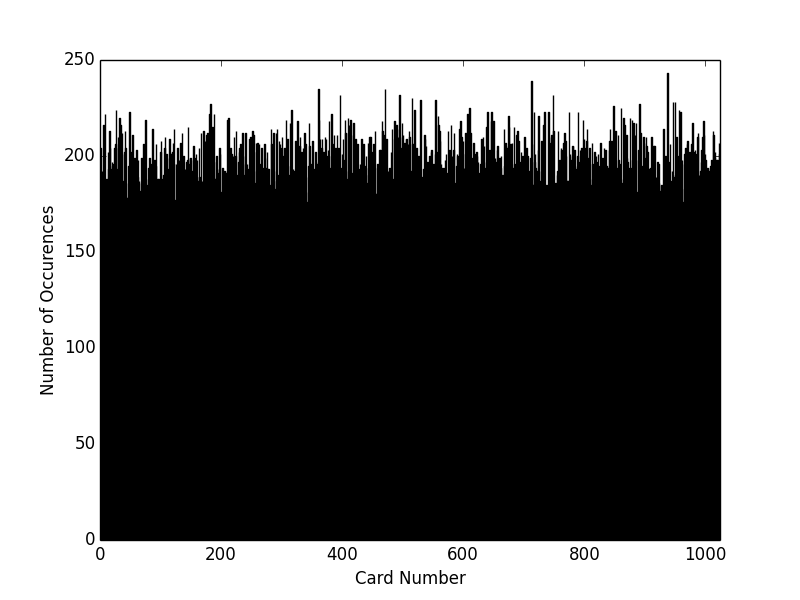
\includegraphics[width=.75\linewidth]{4p5v10000Init.png}
\caption{4 properties, 5 values, 10,000 trials Initial Board Distribution}
\label{fig:init2}
\end{minipage}
\end{figure}


The distribution of cards drawn (excluding the starting board only isolating the $v$ cards drawn) also forms a uniform distribution as can be seen in Figure~\ref{fig:draw1}  and~\ref{fig:draw2}, when the boards have 3 properties, 4 values or 4 properties, 5 values over 10,000 trials. Therefore, this confirms that the implementation of the Fisher Yates shuffle in creating a perfectly random board and draws was successful. 

\begin{figure}[htbb]
\begin{minipage}[b]{0.5\linewidth}
\centering
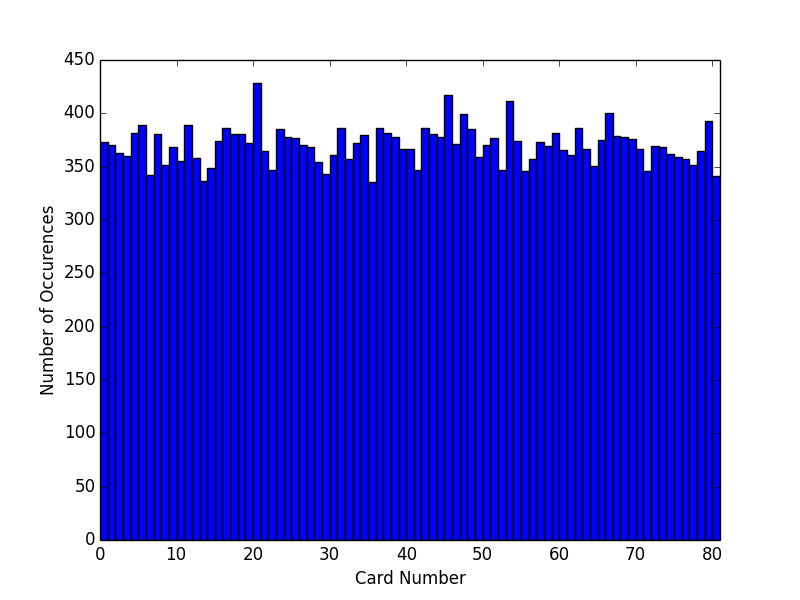
\includegraphics[width=.75\linewidth]{3p4v10000Draw.png}
\caption{3 properties, 4 values, 10,000 trials Distribution of $4$ New Cards Drawn}
\label{fig:draw1}
\end{minipage}
\hspace{0.5cm}
\begin{minipage}[b]{0.5\linewidth}
\centering
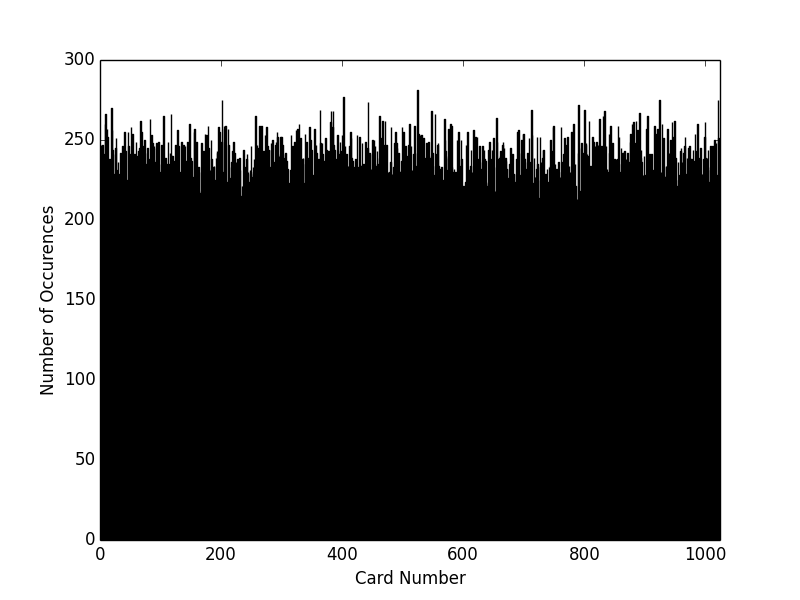
\includegraphics[width=.75\linewidth]{4p5v10000Draw.png}
\caption{4 properties, 5 values, 10,000 trials Distribution of $5$ New Cards Drawn}
\label{fig:draw2}
\end{minipage}
\end{figure}





\subsection{Brute Force Implementation}

As a very naive implementation, I implemented a Brute Force solution that tests all possible combinations of $v$ cards till a set is found and returns this set. A maximum total number of ${v*p}\choose{3}$ sets will have to be examined before a set is found. This can be carried out $n$ times to find $n$ sets and therefore does not build on any previous knowledge, completely checking all possible sets each iteration, though it may have checked the possible set in a previous search. Though not optimized in anyway, the Brute Force implementation provides a benchmark algorithm to compare the SMT based and Dynamic Algorithm based algorithm against. 

\subsection{SMT Solver Implementation}


\subsubsection{Z3:}
I used Z3, a high performance theorem prover created by Microsoft Research. The software creates an easy way to create variables and constraints in Python. Each card that needs to be found represents $p$ variables. I coded the above constraints in Z3 and if the SMT solver outputs "sat," then we know there exists a satisfying set of assignments for the variables that will can be satisfied under the constraints. Therefore, this satisfying assignments represents the $v$ cards, or $v*p$ total variables, that compose a set. If the SMT solver is "unsat," then there exists no satisfying assignment and more cards must be drawn to find a set. 

% Once a set has been found,  I then queue the set to be removed, with all preceding sets to be removed if there exists any. This would take advantage of the fact that if there exists many sets on the board, then the SMT solver would only add constraint 14 to negate any cards of the satisfying set to be one of the cards already found to be a part of set. This would provide a marginal speedup, but is important for creating a fast as possible benchmark for the dynamic algorithm to compete against. 

\subsubsection{Delayed Deletion Optimization:}

To optimize the SMT Solver implementation, I queue up the set to be removed and add the constraints defined in constraint 14 to run through the SMT Solver again to find another set to be removed in case there existed many sets already on the starting board. Once the SMT Solver no longer says that with the constraints and variables it is satisfied, I then know to add $v$ new cards (or more if the board had a lot of sets and therefore the SMT solver was able to find my sets without having to update the constraints) to hopefully create a new set. I will only do this once no sets exist on the board after removing so many cards to hopefully provide marginal speedup to the program. Also, the cards need to be deleted from the board and therefore, I will call upon the Randomizer method to delete all the cards found by the SMT before no sets existed on the board. Therefore, this will make sure that the dynamic algorithm doesn't have too much of a lead when removing cards. Now, I will add $v$ new cards and rebuild the constraints (7, 9, 11) and run the SMT solver to hopefully find another set of cards. 

This iterative sequence will take place $n$ times to find $n$ sets within a game and the SMT solver will return these sets for validation of a legal set. 

\subsubsection{Constraining the Domain Optimization:}

The SMT solver iteratively searches for a solution through a search tree, attempting to constrain the domain for each variable until a satisfying assignment has been discovered, a process called Forward Checking, or all the possible assignments have been exhausted and the constraints cannot be satisfied  \cite{search_from_AI}. Therefore, without constraint 13, the satisfying assignment can be achieved through any permutation of cards of a set and the domain would be much larger to be searched through. The SMT solver will be forced to check every permutation of cards for a set, when in reality, all permutations of a given set are equivalent because order does not matter in a set of cards to satisfy the constraints. To break this symmetry for multiple sets, constraint 13 enforces that the cards in a set are in sorted order (ie. by the first property or if all equal then by the second property and so forth for all properties) and constrains the domain of each variable. This will break the symmetry in the encoding and speed up the process of the SMT solver, as the SMT solver will not need to search branches of its search tree that are duplicates of another branch. 

\subsection{Dynamic Algorithm Implementation}

The Dynamic Algorithm approach hinges on the tradeoff between memory and speed. The Brute Force solution does not need to keep track of partial sets and can spend time iterating over all combos as fast possible. The SMT solver computes a set even faster by pruning the search as it continues through the algorithm to create marginal speed up while recording down possible search paths and deleting branches that have no chance of yielding a correct solution. And in the extreme case, the Dynamic Algorithm will utilize more space, recording down possible sets that can be quickly completed when new card are drawn. Therefore, the Dynamic Algorithm can complete sets in almost instantaneous time when large numbers of sets are to be found and when there is a low chance of there being a set in the board at a given time. 

The Dynamic Algorithm's main speedup is in the way that it creates a list of partial sets and a dictionary mapping the missing card to an almost complete partial set so it can quickly finish these sets when new cards are drawn. 

\subsubsection{Set Up}

To create all partial sets, the Dynamic approach begins similarly to the brute force solution. When the board is created, the solver will initially create partial sets for all ${v*p}\choose{2}$ using Python's built in itertools library since a possible set can be wholly determined by two cards(ie. if the first two cards have the same value for a given property, the satisfying cards must have the same value for that property). These two card partial sets will be the basis for creating larger partial sets and will ensure that all combinations of cards are checked for completing a set. 

\subsubsection{Partial Set List and Quick Complete Dictionary Creation}

Next, for each partial set, the algorithm will determine which cards to add to the partial set from the board that satisfy the constraints that for each property, the values are either the same or all different and must not be in the set of cards that we flag as unusable cards as they have been used to complete a set in a previous iteration. At the end of iterating over all cards on the board, there are two important cases that a partial set could be in:

\textbf{Case 1: Size $v$:} If the partial set is completely full and at size $v$, then the partial set is a complete satisfying set and can therefore be queued as a found set. These cards will also be queued up as cards that will need to be deleted from the partial sets and board and cannot be used to complete other partial sets.

\textbf{Case 2: Size $v-1$:} This partial set is missing one card that can be determined by the rest of the cards in the partial set as the value will be the same if the set has the same value for a given property and if they are all different then it will be the last missing value. Therefore, to create the quick complete data structure, I add to the dictionary the missing card mapped to the partial set. 

Otherwise, the partial set is not complete enough to create a data structure for and therefore will be left. This process will continue for all partial sets. 


\subsubsection{Quick Complete Upon Drawing Cards}

When more sets are needed to be found than exist on the board, new cards must be drawn to create opportunity for more sets. When these $v$ new cards are drawn, the dynamic algorithm will use its quick complete dictionary to quickly search to see if any of the $v$ cards drawn satisfy and of the partial sets that are missing one card. If they complete a partial set, the dictionary will delete the card from the dictionary, append it to the partial set it completes, and add it to the queue of found cards. As we iterate through, it is possible that the cards used in one of these quick completed sets could be used for another completed set and therefore we need to iterate through the cards in a possibly quick completed set to make sure that it was not used to complete a previous set. 

After we have completed all of the partial sets we could have with the new drawn cards, we must create new basis partial sets from these new cards that remain not completing any partial set. Therefore, I again use the itertools library and use combinations to append all combinations of two cards from the unused new cards drawn, and append these to the list of partial sets. With these new partial sets appended, the program then reruns the algorithm described above (5.4.2) to append new cards from the board onto the partial sets, potentially complete sets using a combination of the cards drawn, and add new entries to the quick complete dictionary if necessary. 

\subsubsection{Deletion Bookkeeping}

After both of the above steps, we need to ensure that any set found is appropriately removed from the partial sets. Therefore, I iterate over all partial sets and see if any of them contain a card that was used to complete a set. If it does, I delete the card from the partial set. After we iterate through all of the partial sets, any partial set that is now of length one or zero is no longer a partial set as either it no longer contains any cards or it non longer has specific cards it is searching for since a set needs two cards to determine what cards it is searching for.

I also iterate over the quick complete dictionary and see whether any of the almost completed, partial sets contain the cards we are removing. If they do, we must delete it from the dictionary as it is now missing more than one card which was the criteria to be included in the quick complete dictionary. Once we have deleted the cards from the appropriate data structures, we can iteratively continue these steps until $n$ sets have been found. 

\subsection{Testing}

For both of these implementation, I will need to implement testing to ensure that the sets found by the solvers are indeed sets and that the algorithm correctly removed the sets from the board. 

\subsubsection{Testing Satisfying Set}

To confirm that for all properties the cards from the set have either the same value or all different value, I iterated over all properties and all cards values of that property to check whether when put into a set data structure that the length of the set was either 1, meaning that all the values were the same, or the same length as before, meaning all values were distinct elements. 

To check that all the boards must be from the board, I had to store all iterations of the board, as new cards could be added and sets would be removed. Therefore, I used a set data structure to store all the cards, and updated this set as new cards were added to the board. Finally, I iterated over each set found and checked that it was included in the board at some point and therefore meant it was taken from the board. 

To confirm that the last constraint of all distinct cards was satisfied for each possible set, I asserted that the length of the set was equivalent to the length of the set when converted into a set data structure. Therefore, if they are equal, all elements in the set are therefore distinct and make up all different cards.

Finally, the solver has to handle finding many sets, and to ensure that the solver does not find the same set $n$ times, I assert that when converted to a long list of cards that make up all $n$ sets found, that the length of this list converted to a set data structure should be the same as the length of the long list. Therefore, it would show that all $n*v$ cards are all distinct. 

\subsubsection{Testing Correct Deletion}

The constraints created for the SMT solver also relies on the fact that the cards from a satisfying set must be deleted from the board at some point. Therefore, as a check to ensure that the corresponding cards were deleted from the board set, I iterated over all cards and asserted that all the cards found as part of sets were no longer part of the board at termination of the program. This is a good double check to ensure that SMT solver is functioning properly, because the SMT hinges on the fact that the cards that can no longer be used are to be deleted from the board for rebuilding the corresponding constraints. This is also important for the Dynamic solver and Brute Force implementation because they must output the correct board as well after finding $n$ sets. At termination, we iterate over all cards found as being part of sets and assert that they are no longer part of the board.


\section{Results}

\subsection{Testing Structure}

To test the relative effectiveness of the three implementations, I divided the testing into three different cases to see how the implementations functioned on a variety of test cases. Since there are three variables to change, number of values, properties, and sets to find, I vary one of them and keep the other two constant . This creates a total of three overarching categories that can be broken down into multiple categories as the two constant variables can take on different values and have the third value vary. 

To accurately test the timing of each solver, I utilized Python's time library to accurately test CPU time used for each of the processes. Therefore, if other processes are running in the background and take some real time, this will not factor into the timing tests of these solvers. Also, only the process of creating the solver data structure and finding $n$ sets is accounted as CPU time, as creating the randomizer and verification of correct sets following finding the sets is irrelevant to the speed of the solver itself. 

To give more accurate results, the times for a given set of values, properties, and sets to find are averaged over ten trials to give one data point. Therefore, this would account for instances in which a set can be found instantly or if all combinations need to be examined to find a set, and would give a more accurate picture of an accurate test case. Also, before each one of these ten trials, a new board is created by instantiating a new randomizer such that the solver will not be redoing the same computation it had just finished. 

I again used a Python package called matplotlib to graph all of the curves formed from the timing tests. These graphs are composed of connected dotted lines that are color coded by solver, red to Brute Force, blue to SMT, and green to Dynamic solver, and give an easy to read visualization of order of growth as a variable is changed. 


\subsection{Varying the Number of Values}

In the case of changing the value of the deck to be used, the value has to be restricted to be greater than two. If the number of values was either one or two, then a set could be immediately found as any card and any two cards are a valid set, in each case respectively. Therefore, I only test values in which the are larger than two for accurate results. 


\begin{table}[hbt]
  \centering
  \begin{tabular}{|l|l|}
    \hline
    \textbf{Field} & \textbf{Value}\\
    \hline
    \hline
    Paper size & US Letter 8.5in $\times$ 11in\\
    \hline
    Top margin & 1in\\
    \hline
    Bottom margin & 1in\\
    \hline
    Left margin & 1in\\
    \hline
    Right margin & 1in\\
    \hline
    Body font & 12pt\\
    \hline
    Abstract font & 12pt, italicized\\
    \hline
    Section heading font & 14pt, bold\\
    \hline
    Subsection heading font & 12pt, bold\\
    \hline
  \end{tabular}
  \caption{Formatting guidelines. }
  \label{table:formatting}
\end{table}

\begin{table}[hbt]
  \centering
  \begin{tabular}{|l|l|} \hline
    \textbf{Some field} & \textbf{Another field}\\\hline
    200          &  10000 \\ \hline 
    400          &  20000 \\ \hline 
    800          &  40000 \\ \hline 
    1600        &  80000 \\ \hline 
    3200        &  160000 \\ \hline 
    6400        &  320000 \\ \hline 
  \end{tabular}
  \caption{Some data in a table. }
  \label{table:data}
\end{table}


\subsection{Varying the Number of Properties}

\subsection{Varying the Number of Sets to be Found}





Changing Values:


Changing Properties:




Changing Number of Sets to Find:

Over 10 trials
Value: 3 | Properties: 4 | Sets found: 2 | SMT time: 0.0830945 | Dynamic time: 0.0012532 | Brute Force time: 0.0792278
Value: 3 | Properties: 4 | Sets found: 3 | SMT time: 0.1309777 | Dynamic time: 0.0021258 | Brute Force time: 0.1288052
Value: 3 | Properties: 4 | Sets found: 4 | SMT time: 0.1469017 | Dynamic time: 0.00206 | Brute Force time: 0.1598722
Value: 3 | Properties: 4 | Sets found: 5 | SMT time: 0.1981986 | Dynamic time: 0.0031261 | Brute Force time: 0.2002846
Value: 3 | Properties: 4 | Sets found: 6 | SMT time: 0.2494722 | Dynamic time: 0.0051556 | Brute Force time: 0.2630714

Over 5 trials
Value: 4 | Properties: 5 | Sets found: 2 | SMT time: 0.8491608 | Dynamic time: 0.2452296 | Brute Force time: 1.1175872
Value: 4 | Properties: 5 | Sets found: 3 | SMT time: 1.7955682 | Dynamic time: 0.2946156 | Brute Force time: 1.1840924
Value: 4 | Properties: 5 | Sets found: 4 | SMT time: 1.930447 | Dynamic time: 0.4328736 | Brute Force time: 1.7126942
Value: 4 | Properties: 5 | Sets found: 5 | SMT time: 2.4920082 | Dynamic time: 0.3662846 | Brute Force time: 2.5330248
Value: 4 | Properties: 5 | Sets found: 6 | SMT time: 2.2934102 | Dynamic time: 0.4965884 | Brute Force time: 2.2322826

\section{Conclusion}









\subsection{Paper Formatting}
\label{section:formatting}

There are no minimum or maximum length limits on IW reports.  
We are including this template because we think it will be helpful
for citing things properly and for including figures into formatted
text.  If you are using \LaTeX~\cite{lamport94} 
to typeset your paper, then we strongly suggest
that you start from the template available at
http://iw.cs.princeton.edu -- this
document was prepared with that template.  
If you are using a different software package to typeset your paper, 
then you can still use this document as a reasonable sample of 
how your report might look.  Table~\ref{table:formatting} is a suggestion
of some formatting guidelines, as well as being an example of how to
include a table in a Latex document.

\begin{table}[hbt]
  \centering
  \begin{tabular}{|l|l|}
    \hline
    \textbf{Field} & \textbf{Value}\\
    \hline
    \hline
    Paper size & US Letter 8.5in $\times$ 11in\\
    \hline
    Top margin & 1in\\
    \hline
    Bottom margin & 1in\\
    \hline
    Left margin & 1in\\
    \hline
    Right margin & 1in\\
    \hline
    Body font & 12pt\\
    \hline
    Abstract font & 12pt, italicized\\
    \hline
    Section heading font & 14pt, bold\\
    \hline
    Subsection heading font & 12pt, bold\\
    \hline
  \end{tabular}
  \caption{Formatting guidelines. }
  \label{table:formatting}
\end{table}

\textbf{Please ensure that you include page numbers with your
submission}. This makes it easier for readers to refer to
different parts of your paper when they provide comments.

We highly recommend you use bibtex for managing your references and citations.  You can add bib entries to a references.bib file throughout the semester (e.g., as you read papers) and then they will be ready for you to cite when you start writing the report.  If you use bibtex, please note that the references.bib file provided in the template example includes some format-specific incantations at the top of the file.  If you substitute your own bib file, you will probably want to include these 
incantations at the top of it.

\subsection{Citations and Footnotes}

There are various reasons to cite prior work and include it as references in your bibliography.  For example, If you are improving upon 
prior work, you should include
a full citation for the work in the bibliography \cite{nicepaper,nicepaper2}. 
You can also cite information that is used as background or
explanation\cite{Salzberg:2005}.  In addition to citing scholarly papers or books, you can
also create bibtex entries for webpages or other sources.  Many online
databases allow you to download a premade bibtex entry for each paper
you access.  You can simply copy-paste these into your references.bib
file.

Sometimes you want to footnote something, such as a web
site.\footnote{http://www.cs.princeton.edu}  Note that the footnote
number comes after the punctuation.

\subsection{Figures and Tables.}

Figure \ref{fig:gray} shows an example of how to include a figure in
your report.  
Ensure that the figures and
tables are legible.  Please also ensure that you refer to your
figures in the main text. Make sure that your figures will be legible
in the expected forms that the report will be read.  If you expect someone
to print it out in gray-scale, then make sure the figures are legible 
when printed that way.  

\begin{figure}[hbt]
\centering

\includegraphics[width=0.75\linewidth]{gray.jpg}
\caption{This is a gray image.}
\label{fig:gray}
\end{figure}

In Section~\ref{section:formatting}, an example of a table was given.
(Note that the ``S'' in Section is capitalized.  Here's one more
example - see Table~\ref{table:data}.

\begin{table}[hbt]
  \centering
  \begin{tabular}{|l|l|} \hline
    \textbf{Some field} & \textbf{Another field}\\\hline
    200          &  10000 \\ \hline 
    400          &  20000 \\ \hline 
    800          &  40000 \\ \hline 
    1600        &  80000 \\ \hline 
    3200        &  160000 \\ \hline 
    6400        &  320000 \\ \hline 
  \end{tabular}
  \caption{Some data in a table. }
  \label{table:data}
\end{table}


Here's an example that shows how you can have side-by-side figures -
see Figure~\ref{fig:side-a} and Figure~\ref{fig:side-b}.  (Note that
the the ``F'' in Figure is capitalized. 

\begin{figure}[htbb]
\begin{minipage}[b]{0.5\linewidth}
\centering

\includegraphics[width=.75\linewidth]{checkerboard-squares-black-white.jpg}
\caption{Plain checkerboard.}
\label{fig:side-a}
\end{minipage}
\hspace{0.5cm}
\begin{minipage}[b]{0.5\linewidth}
\centering

\includegraphics[width=.75\linewidth]{swirl-squares-black-white.jpg}
\caption{Cool checkerboard.}
\label{fig:side-b}
\end{minipage}
\end{figure}

\subsection{Double Quotes.}

Latex double quotes are not the same as the double quote key on your
keyboard. The standard way of writing quotes and double quotes in
LaTeX is with `` and '' not with " and ".   

Now that may be confusing, so you may want to use the \textbackslash\{quotes\} command.  For
example \quotes{The quick brown fox.}



\subsection{Main Body.}

Avoid bad page or column breaks in
your main text, i.e., last line of a paragraph at the top of a
column or first line of a paragraph at the end of a column. If you
begin a new section or sub-section near the end of a column,
ensure that you have at least two (2)  lines of body text on the same
column. 

\section{Outline}  
The following is a possible outline for your paper.
\subsection{Introduction}
\begin{itemize}
\item Motivation and Goal (The goal of this project is...)
\item Overview of challenge and previous work 
\item Approach 
\item Summary of implementation
\item Summary of results
\item (optional) Roadmap: The remainder of this paper is organized as follows....
\end{itemize}

\subsection{Problem Background and Related Work}
\begin{itemize}
\item Survey of prior work with similar goals 
\item For each previous approach, explain what has been done and why it does not meet your goal
\end{itemize}

\subsection{Approach}
\begin{itemize}
\item Key novel idea
\item Why it is a good idea
\end{itemize}

\subsection{Implementation}
\begin{itemize}
\item System overview (flow chart of key steps?)
\item Subsection for each step or issue you addressed
\begin{itemize}
\item Problem statement
\item Possible approaches
\item Chosen approach and why
\item Implementaton details
\end{itemize}
\end{itemize}

\subsection{Evaluation}
\begin{itemize}
\item Experiment design...
\item Data...
\item Metrics...
\item Comparisons...
\item Qualitative results...
\item Quantitative results...
\end{itemize}

\subsection{Summary}
\begin{itemize}
\item Conclusions...
\item Limitations...
\item Future work...
\end{itemize}


\section{Ethics}

Your independent work report should abide by the basic standards of scholarly ethics and by the Princeton Honor Code. If you have any doubts about how to cite
other work, how to quote or include text or images from other works, or other issues, please discuss them with your project adviser or with the IW coordinators. 



\bstctlcite{bstctl:etal, bstctl:nodash, bstctl:simpurl}
\bibliographystyle{IEEEtranS}
\bibliography{references}

\end{document}

